\documentclass[12pt]{article}

\usepackage[a4paper, total={6in, 8in}]{geometry}
% \usepackage{textcomp}

\usepackage{listings}
\usepackage{color}
\usepackage{graphicx}
\graphicspath{ {../images/} }


\definecolor{dkgreen}{rgb}{0,0.6,0}
\definecolor{gray}{rgb}{0.5,0.5,0.5}
\definecolor{mauve}{rgb}{0.58,0,0.82}

\lstset{frame=tb,
  language=Python,
  aboveskip=3mm,
  belowskip=3mm,
  showstringspaces=false,
  columns=flexible,
  basicstyle={\small\ttfamily},
  numbers=none,
  numberstyle=\tiny\color{gray},
  keywordstyle=\color{blue},
  commentstyle=\color{dkgreen},
  stringstyle=\color{mauve},
  breaklines=true,
  breakatwhitespace=true,
  tabsize=3
}

\title{Apt-Zücher}
\author{Eugenio Barbieri Viale}
\date{12 maggio 2025}

\begin{document}
\setlength{\parindent}{0pt}

\maketitle
Il progetto consiste di due programmi in Python:
\begin{verbatim} main.py \end{verbatim} 
\begin{verbatim} webscrape.py \end{verbatim}
Il primo elabora i dati, genera i grafici e la lista degli appartamenti migliori. \\
Il secondo ricava le informazioni degli appartamenti dal sito \textit{homegate.ch} e per ognuno calcola la distanza dall'ETH, grazie alle coordinate GPS ottenute dall'indirizzo.

\newpage
Gli appartamenti di cui non è stato possibile ricavare le informazioni sono rappresentati nel grafico con il valore $0$.

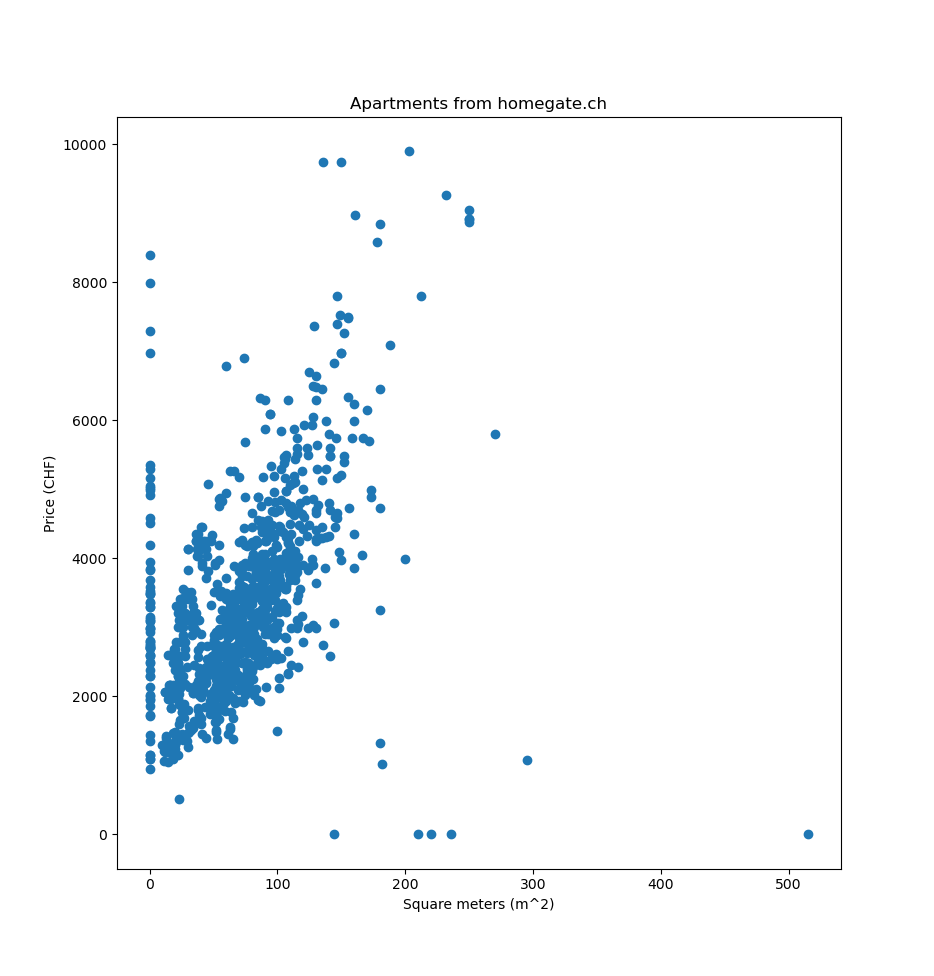
\includegraphics[scale=0.65]{homegate_meters}

È possibile notare che all'aumentare dei metri quadri aumenta anche il prezzo, come ci si aspetterebbe. Il tipo di andamento che meglio descrive questa tendenza potrebbe essere lineare.

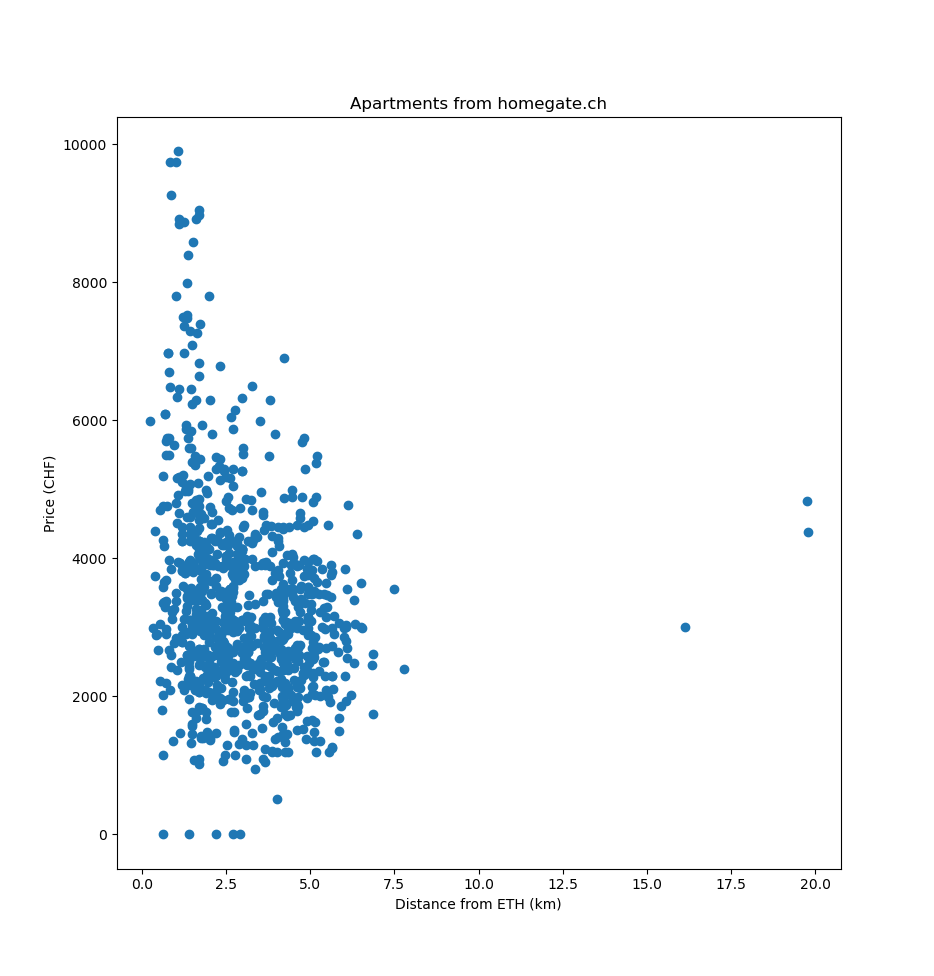
\includegraphics[scale=0.65]{homegate_distances}

Si può vedere che purtroppo gli appartamenti più costosi sono anche quelli più vicini all' ETH.

\newpage
\begin{verbatim}
main.py
\end{verbatim}

\lstset{language=Python}
\begin{lstlisting}
from os import path
from time import sleep

import pandas as pd
import matplotlib.pyplot as plt
from numpy import array, argsort

import webscrape

dirname = "data"

filename = dirname + "/homegate.csv"

if not path.isfile(filename):
    w = webscrape.WebScrape(None, None)
    w.write_data(start_page=1, end_page=51, timeout=7, path=filename, show=True)

prices = pd.read_csv(filename, usecols=["price"]).values
rooms = pd.read_csv(filename, usecols=["rooms"]).values
meters = pd.read_csv(filename, usecols=["meters"]).values
addresses = pd.read_csv(filename, usecols=["address"]).values

dist_file = dirname + "/distances.csv"

if not path.isfile(dist_file):
    w = webscrape.WebScrape(None, None)
    w.write_distances(addresses, path=dist_file, timeout=1.1, show=True)

distances = pd.read_csv(dist_file, usecols=["distance"]).values

def price_meters_graph():
    plt.title("Apartments from homegate.ch")
    plt.xlabel("Square meters (m^2)")
    plt.ylabel("Price (CHF)")

    plt.scatter(meters, prices)
    plt.show()

def price_dist_graph():
    plt.title("Apartments from homegate.ch")
    plt.xlabel("Distance from ETH (km)")
    plt.ylabel("Price (CHF)")

    plt.scatter(distances, prices)
    plt.show()


def loss(p, m, r, d, weights):
    if p != 0.0 and m != 0.0 and r != 0.0:
        return (p * weights[0] / (m * weights[1])) + (d * weights[2] /  (r * weights[3]))
    return 10.0

limit_price = 4000
limit_rooms = 3.0

lst_prices = []
lst_meters = []
lst_rooms = []
lst_distances = []

targets = []
for i in range(len(prices)):
    if prices[i] <= limit_price and rooms[i] >= limit_rooms:
        targets.append([prices[i], meters[i], rooms[i], addresses[i], distances[i]])

        lst_prices.append(prices[i][0])
        lst_meters.append(meters[i][0])
        lst_rooms.append(rooms[i][0])
        lst_distances.append(distances[i][0])

max_price = max(lst_prices)
max_meter = max(lst_meters)
max_room = max(lst_rooms)
max_distance = max(lst_distances)

# price, meters, rooms, distance
weights = [0.4, 0.7, 0.9, 0.4]

scores = []
for i in range(len(targets)):
    p = float(lst_prices[i]) / float(max_price)
    m = float(lst_meters[i]) / float(max_meter)
    r = float(lst_rooms[i]) / float(max_room)
    d = float(lst_distances[i]) / float(max_distance)

    score = loss(p, m, r, d, weights)
    scores.append(score)

np_scores = array(scores)
sorted_indices = np_scores.argsort()
sorted_scores = np_scores[sorted_indices]

for i in range(10):
    best_apartment = targets[sorted_indices[i]]
    print("Score:", round(sorted_scores[i], 2), best_apartment[0][0], best_apartment[1][0], best_apartment[2][0], best_apartment[3][0], best_apartment[4][0])

\end{lstlisting}

\newpage
\begin{verbatim}
webscrape.py
\end{verbatim}

\lstset{language=Python}
\begin{lstlisting}
import requests
from time import sleep
from bs4 import BeautifulSoup
from csv import writer
from geopy.geocoders import Nominatim
from geopy import distance
from geopy.exc import GeocoderTimedOut


class WebScrape:
    def __init__(self, price, rooms):
        self.price = price
        self.rooms = rooms

        self.site_url = "https://www.homegate.ch/rent/apartment/city-zurich/matching-list"

        self.headers = { 'User-Agent': 'Mozilla/5.0 (Windows NT 10.0; Win64; x64) AppleWebKit/537.36 (KHTML, like Gecko) Chrome/58.0.3029.110 Safari/537.3'}

    def reach_site(self, page):
        url = self.site_url + "?ep=" + str(page) + "&ac=" + str(self.rooms) + "&ipd=false" + "&ah=" + str(self.price)
        s = requests.Session()

        try:
            r = s.get(url, headers=self.headers)
            print(r)

        except requests.exceptions.Timeout as ex:
            print("Exception raised: ", ex)

        soup = BeautifulSoup(r.content, "html.parser")
        self.infos = soup.find_all("div", attrs={"class": "HgListingCard_info_RKrwz"})

    def get_space(self, info):
        space = info.find("div", class_="HgListingRoomsLivingSpace_roomsLivingSpace_GyVgq").get_text()

        rooms = []
        for i in range(len(space)):
            if i <= 4:
                if space[i].isdigit() or space[i] == ".":
                    rooms.append(space[i])
            else:
                rooms = "".join(rooms)
                break

        meters = []
        for i in range(7, len(space)):
            if space[i].isdigit() and space[i] != "²":
                meters.append(space[i])

        meters = "".join(meters)

        if "²" in rooms:
            meters = rooms.replace("²", "")
            rooms = 0

        if meters == "" or meters == []:
            meters = 0

        if rooms == "" or rooms == []:
            rooms = 0

        return float(rooms), int(meters)

    def get_price(self, info):
        price = info.find("span", class_="HgListingCard_price_JoPAs").get_text()[4:10].replace(",", "")

        if price == "ce on ":
            return 0

        price = "".join(c for c in price if c.isdigit())

        return int(price)

    def write_data(self, start_page=1, end_page=51, timeout=2, path="data.csv", show=None):
        self.data = [
            ["price", "rooms", "meters", "address"]
        ]

        for page in range(start_page, end_page):
            print(f"\n------- PAGE NUMBER {page} -------")

            self.reach_site(page)

            for info in self.infos:
                price = self.get_price(info)
                rooms, meters = self.get_space(info)
                address = info.find("address", attrs={"translate": "no"}).get_text()
                
                t = [price, rooms, meters, address]
                self.data.append(t)

                if show == True:
                    print(t)

            sleep(timeout)

        with open(path, mode="w", newline="") as file:
            w = writer(file)
            w.writerows(self.data)

        print(f"CSV file '{path}' created successfully")

    def get_coords(self, address):
        geolocator = Nominatim(user_agent="myapp")

        try:
            target = geolocator.geocode(address, timeout=None)
            destination = geolocator.geocode("Rämistrasse 101 8092 Zurich", timeout=None) # eth address
            return target, destination

        except GeocoderTimedOut:
            return self.get_coords(address)

    def get_distance(self, address):
        target, destination = self.get_coords(address)

        if target == None:
            return -1.0

        gps_targ = (target.latitude, target.longitude)
        gps_dest = (destination.latitude, destination.longitude)

        dist = distance.geodesic(gps_dest, gps_targ).km
        return round(dist, 2)

    def write_distances(self, addresses, path="data/distances.csv", timeout=7, show=True):
        distances = [
                ["distance"]
        ]
        i = 0

        for address in addresses:
            distance = self.get_distance(address)
            distances.append([distance])

            if show == True:
                print(i, address, distance)

            sleep(timeout)
            i += 1
        
        with open(path, mode="w", newline="") as file:
            w = writer(file)
            w.writerows(distances)

        print(f"CSV file '{path}' created successfully")
\end{lstlisting}

\end{document}
